% ED-23 -- The isothermal theorem of evolutionary graph theory, kernel-checked
% Sources: TOP20.json pick 7; papers/p3_isothermal_theorem/{AUDIT.md,REVISION.md,publication_meta.json}
% Figure: code/fig07.py -> figures/c07_graphes.{pdf,png}
\chapter[Le plan de table et la sélection]{Quand le plan de table ne change rien à la sélection}
\reference{Préprint du 26 octobre 2026.\\ doi:10.5281/\\zenodo.23660071}

\section*{L'idée en une image}

\begin{analogie}
Une grande tablée, une chaise par convive. À chaque manche, un convive est tiré au sort, avec plus de chances s'il
est \og fort\fg{} (le mutant compte $r$ fois plus qu'un convive ordinaire), et il installe un de ses disciples sur une
chaise que le plan de table lui désigne, à la place de son occupant. Le plan de table, c'est un réseau~: il dit qui
peut remplacer qui, et avec quelle chance. Le théorème dit ceci~: si \emph{chaque chaise est remplacée aussi
souvent que les autres}, le plan de table, aussi tordu soit-il, ne change rien à la chance qu'a un clan de finir par
occuper toute la table. Tout se passe comme si les convives étaient bien mélangés.

\emph{Où l'image cesse d'être juste~:} le résultat vaut pour cette règle précise (d'abord on choisit qui se
reproduit, ensuite qui est remplacé)~; avec la règle inverse, ou si l'on parle de vitesse plutôt que de chance
finale, rien n'est démontré ici.
\end{analogie}

\section*{Ce qui a été fait}

En théorie de l'évolution sur réseaux, la population est posée sur les sommets d'un graphe. Une matrice $W$ donne,
pour chaque individu $i$, la chance $W_{ij}$ que son descendant remplace l'individu $j$~; chaque ligne de $W$ fait
$1$. Le réseau est dit \og isotherme\fg{} quand chaque colonne fait aussi $1$~: chaque individu est remplacé, en
moyenne, au même rythme. Le théorème classique dit qu'alors, si le réseau est d'un seul tenant (on peut aller de
n'importe quel sommet à n'importe quel autre), la chance d'envahir est exactement celle du modèle de Moran, où la population
est bien mélangée~: $(1-r^{-k})/(1-r^{-n})$ pour $k$ mutants parmi $n$.

L'article démontre ce sens du théorème dans Lean, ainsi qu'une généralisation où les individus reçoivent des
poids de reproduction différents mais \og à l'équilibre\fg{} avec le réseau. Il réutilise tel quel le théorème
d'absorption du travail sur les probabilités de fixation (doi:10.5281/zenodo.23653850). Et il commence par un aveu~: la formulation annoncée avant le travail, \og le
nombre de mutants évolue comme une simple échelle\fg, est \emph{fausse} pour la chaîne étudiée. Ce qui est vrai, et
démontré, est plus fin~: dans \emph{chaque} configuration, la chance de gagner un mutant vaut $r$ fois la chance
d'en perdre un.

\begin{encadre}
\textbf{À faire avec un crayon.} Quatre convives en cercle, numérotés $0,1,2,3$~; chacun remplace l'un de
ses deux voisins, avec une chance $1/2$ chacun. Chaque colonne fait $1$~: le cercle est isotherme. Prenons $r=2$ et
deux mutants. Le poids total est $2+2+1+1=6$.
\begin{itemize}
\item \emph{Mutants voisins, en 0 et 1.} Pour gagner un mutant, il faut que $0$ soit choisi (chance $2/6$) et vise
  son voisin $3$ (chance $1/2$), ou que $1$ vise $2$~: $1/6+1/6=1/3$. Pour en perdre un, il faut que $2$ ou $3$ soit
  choisi ($1/6$ chacun) et vise le mutant voisin ($1/2$)~: $1/12+1/12=1/6$.
\item \emph{Mutants opposés, en 0 et 2.} Chaque mutant n'a que des voisins ordinaires~: gain $2\times2/6=2/3$,
  perte $2\times1/6=1/3$.
\end{itemize}
Avec le même nombre de mutants, les chances diffèrent ($1/3$ ou $2/3$)~: le simple décompte ne suffit pas, d'où
l'erreur de la pré-annonce. Mais le rapport gain/perte vaut $2=r$ dans les deux cas, et c'est ce rapport qui donne
la formule~: $(1-1/2)/(1-1/16)=8/15$ pour un mutant seul. Contre-épreuve~: l'étoile à trois sites (un centre
relié à deux feuilles) n'est pas isotherme. Sa colonne du centre fait $2$ et celle de chaque feuille $1/2$~: le
centre est remplacé deux fois plus souvent que la moyenne, et quatre fois plus souvent qu'une feuille. Un mutant
posé au centre n'envahit qu'avec la chance $5/12$, au lieu de $4/7$~; sur une feuille, $2/3$~; placé au hasard,
$7/12$. Ces trois valeurs sont démontrées dans Lean. La figure~\ref{fig:c07} montre aussi l'étoile à quatre sites
(un centre, trois feuilles), où la population bien mélangée donnerait $8/15$~: le centre n'envahit qu'avec
$392/1265$, une feuille avec $168/253$, un mutant placé au hasard avec $728/1265$. Ces valeurs-là sont seulement
calculées.
\end{encadre}

\begin{figure}[htbp]
\centering
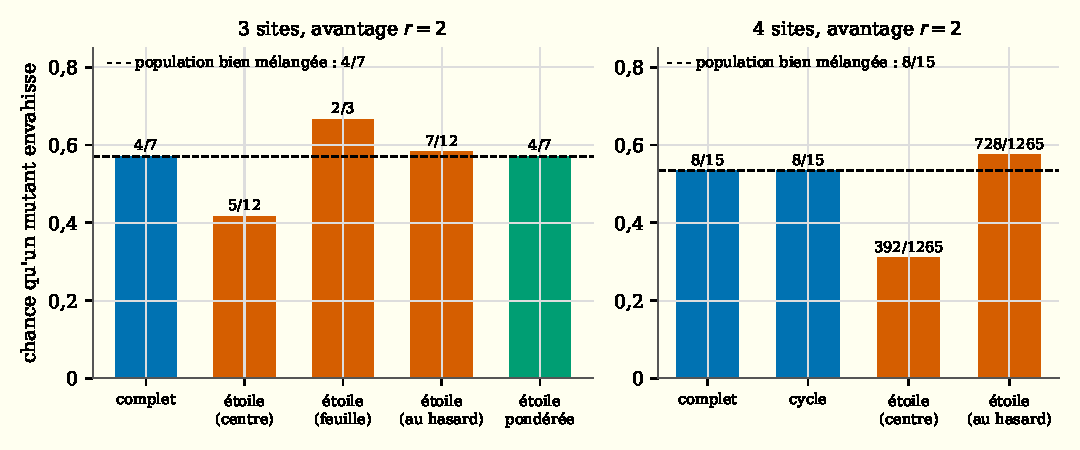
\includegraphics[width=\linewidth]{figures/c07_graphes}
\caption{Chance d'invasion d'un mutant seul, en fractions exactes, à $r=2$~: à gauche trois sites (valeurs démontrées dans Lean), à droite quatre sites (valeurs seulement calculées, niveau~X). Réseaux isothermes en bleu, étoile en orange~; en vert, l'étoile à trois sites avec des poids à l'équilibre, qui retrouve $4/7$.}
\label{fig:c07}
\end{figure}

\section*{Comment on s'est assuré que ce n'est pas faux}

En résumé~: \niveau{A} pour le théorème démontré et pour les valeurs de l'étoile à trois sites, \niveau{C} pour la
lecture biologique, \niveau{X} pour les valeurs numériques de l'étoile à quatre sites de la figure.

Pour le théorème, \og le juge a regardé\fg. Le noyau de Lean, le petit programme qui contrôle chaque pas
logique, a accepté toutes les démonstrations, avec seulement les trois axiomes standard de la liste blanche. Un
auditeur indépendant, un agent d'IA distinct de la même famille de modèles, a tout recompilé dans son propre répertoire,
puis a rejoué chaque déclaration dans le noyau avec un second outil~: sans erreur. Il a recalculé l'étoile et le
cercle avec son propre programme en fractions exactes, et retrouvé les mêmes valeurs.

Il a surtout fabriqué deux fausses preuves, qui devaient échouer. La première, avec un trou bouché par
\texttt{sorry}, se compile sans erreur mais l'audit des axiomes la dénonce. La seconde est plus sournoise~: une
option de débogage qui court-circuite le noyau permet de \og démontrer\fg{} le faux, et la liste des axiomes reste
alors \emph{parfaitement propre}. Seul le rejeu dans le noyau l'a refusée. Leçon reprise dans l'article corrigé~: la
barrière, c'est la liste des axiomes \emph{et} le rejeu \emph{et} la recherche de ces options interdites. Le
registre reste marqué \og non audité\fg~: aucun humain n'a encore vérifié que les énoncés disent ce qu'on croit.

\section*{Ce que ça ne dit pas}

\begin{limite}
\begin{itemize}
\item Seul le sens \og isotherme $\Rightarrow$ comme une population mélangée\fg{} est démontré~; la réciproque ne
  l'est pas.
\item Rien sur les autres règles de mise à jour (d'abord la mort, ensuite la naissance), ni sur des poids qui ne
  forment pas des lignes de somme $1$.
\item \og Chance d'envahir\fg{} veut dire ici la limite d'une puissance de matrice~; le lien avec une loi sur les
  trajectoires est la définition usuelle, non formalisée (\niveau{C}).
\item Les valeurs de l'étoile à quatre sites (figure, à droite) viennent d'un calcul Python en fractions, non
  vérifié par le noyau (\niveau{X})~; celles de l'étoile à trois sites, elles, sont démontrées dans Lean.
\item Aucune nouveauté mathématique n'est revendiquée~: les résultats datent de 2005, 2015 et 2024. Les auteurs ne
  connaissent pas de formalisation antérieure, mais n'ont pas fait de recherche systématique. La portée biologique
  (tissus, amplificateurs de sélection) est une interprétation, sans aucune donnée.
\end{itemize}
\end{limite}

\section*{Pour aller plus loin}

L'article, le verrouillage des énoncés et l'audit sont déposés sous doi:10.5281/\allowbreak zenodo.23660071. Il montre en un
seul document la réutilisation (il importe les briques du travail sur la fixation) et l'humilité (il publie sa propre
erreur de pré-enregistrement).
